\section{Epipolar Geometry}
\subsection*{Epipolar Geometry:} Describes the geometric relationship between two cameras and the corresponding points in their images. 
% It provides constraints that simplify 3D reconstruction and stereo matching. 

1. \textbf{Epipoles:} The intersections of the baseline (the line connecting the two camera centers) with the image planes. Each epipole is the projection of the other camera center. \\
   - All epipolar lines for a given image pass through the epipole. \\
   - Image plane parallel: Epipoles infinitely far away, epipolar lines parallel

   
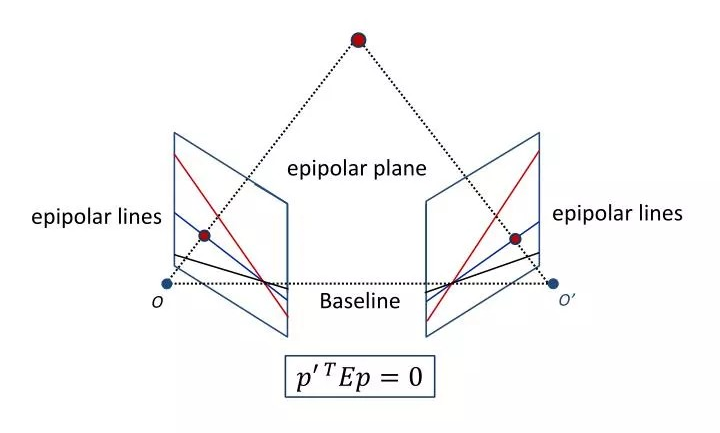
\includegraphics[width=1\linewidth]{images/l12-epipolar.png}
% 3. \textbf{Epipolar Plane:} The plane formed by a 3D point \(X\) and the optical centers of both cameras. Each epipolar plane intersects the two image planes along corresponding epipolar lines. \\

% 4. \textbf{Epipolar Lines:} 
%    - For a point \(p\) in the first image, the corresponding point \(p'\) in the second image must lie on its epipolar line.
%    - This reduces the matching search from 2D to 1D along the epipolar line, greatly simplifying stereo matching. \\

\subsection*{Fundamental and Essential Matrices:}
1. \textbf{Fundamental Matrix \(F\)} relates corresponding points in two \textit{uncalibrated} images, singular(r=2), deg free=7:
     \[
     \mathbf{{p'}}^T F \mathbf{{p}} = 0.
     \]
     It maps a point \(p\) in the first image to its epipolar line in the second image. \\
2. \textbf{Essential Matrix \(E\)} is a special case for \textit{calibrated} cameras:
     \[
     E = [t_x] R,
     \]
     \(R\) : rotation matrix, \([t_x]\) : skew-symmetric matrix representing translation. \\

3. \textbf{Epipolar Constraint (Calibrated Case):}
    With known intrinsic matrices \(K_1\) and \(K_2\), the projection matrices are:
     \[
     M_1 = K_1 [I \mid 0], \quad M_2 = K_2 [R \mid t].
     \]
   % - Given a point \(p\) in the first image, its corresponding point \(p'\) in the second image satisfies:
     \[
     \mathbf{\hat{p'}}^T E \mathbf{\hat{p}} = 0.
     \]
\subsection*{Estimating the Fundamental Matrix}
% 1. \textbf{Objective:} The fundamental matrix \( F \) relates corresponding points between two views in uncalibrated stereo systems. It maps a point \( p \) in the first image to its epipolar line in the second image:
%    \[
%    \mathbf{p'}^T F \mathbf{p} = 0,
%    \]
%    where \( \mathbf{p} = (u, v, 1)^T \) and \( \mathbf{p'} = (u', v', 1)^T \) are corresponding points in homogeneous coordinates. \\

% 2. \textbf{Fundamental Matrix Representation:}
%    - \( F \) is a \( 3 \times 3 \) matrix that encodes the epipolar geometry between two views.
%    - It is rank-deficient (rank 2) and has 7 degrees of freedom. \\

1. \textbf{Linear Estimation of \( F \):}
   From the epipolar constraint and Stacking:

     \[
     u' u f_{11} + u' v f_{12} + u' f_{13} + v' u f_{21} 
     % + v' f_{23} + u f_{31} + v f_{32} + f_{33} = 0.
     \]
     \[
     % u' u f_{11} + u' v f_{12} + u' f_{13} + v' u f_{21} + v' v f_{22} 
     + v' v f_{22}  + v' f_{23} + u f_{31} + v f_{32} + f_{33} = 0.
     \]
     \[
     A \mathbf{f} = 0,
     \]
     where \( A \) is an \( 8 \times 9 \) matrix constructed from the point correspondences, and \( \mathbf{f} \) is the 9-vector representing the entries of \( F \). \\

2. \textbf{Eight-Point Algorithm:}
   - Solve the system \( A \mathbf{f} = 0 \) using Singular Value Decomposition (SVD) to estimate \( F \).
   - \( F \) rank 2, set the smallest singular value of \( F \) to zero. \\

3. \textbf{Normalization:}
   - For better numerical stability:
     \[
     \mathbf{p} \rightarrow \frac{\mathbf{p}}{\|\mathbf{p}\|}, \quad \mathbf{p'} \rightarrow \frac{\mathbf{p'}}{\|\mathbf{p'}\|}.
     \]
   - After the estimation, the fundamental matrix should be denormalized. \\

4. \textbf{RANSAC for Robust Estimation:}
   % - Since real data often includes noise and outliers, the RANSAC algorithm is often used to robustly estimate \( F \).
   - RANSAC randomly samples minimal sets of correspondences (8) to estimate \( F \) and selects the solution that maximizes the number of inliers (pts that satisfy the epipolar constraint within a threshold). \\


% 8. \textbf{Applications of Epipolar Geometry:}
%    - Used in **stereo vision** to recover depth by matching corresponding points along epipolar lines.
%    - Essential for **3D reconstruction**, structure from motion, and camera calibration.
